\subsection{Send message}

\begin{figure}[htb!]
  \centering
    \subfloat[]{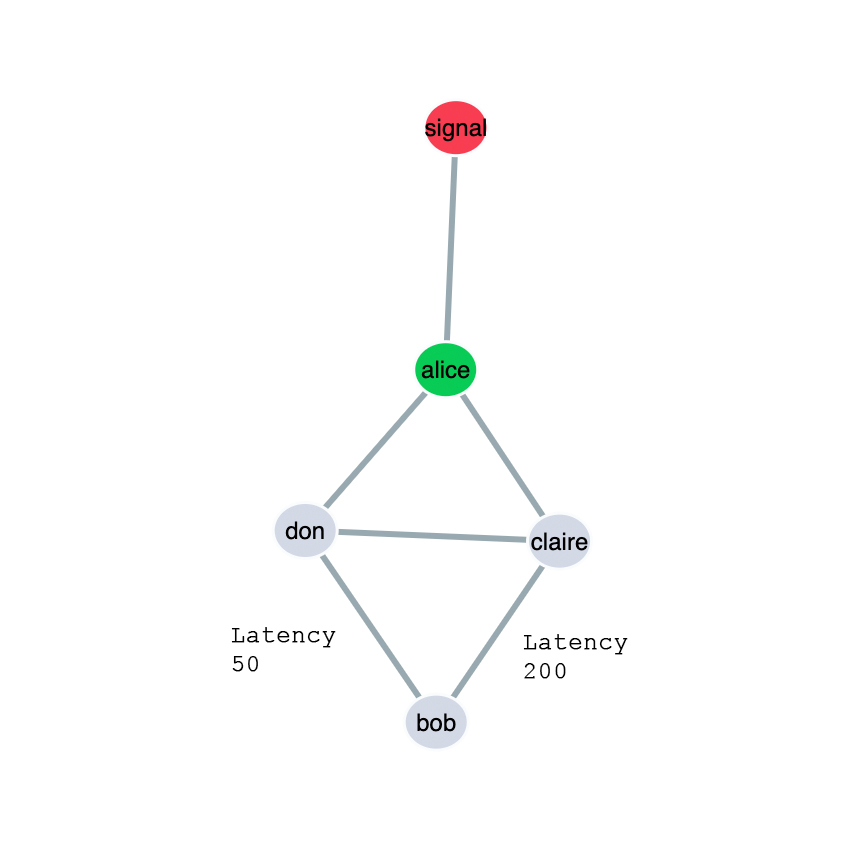
\includegraphics[width=0.25\textwidth]{graphics/analysis/mini-scenarios/send-message/1.jpg} \label{fig:filmstrips-send-message-a}}
    \subfloat[]{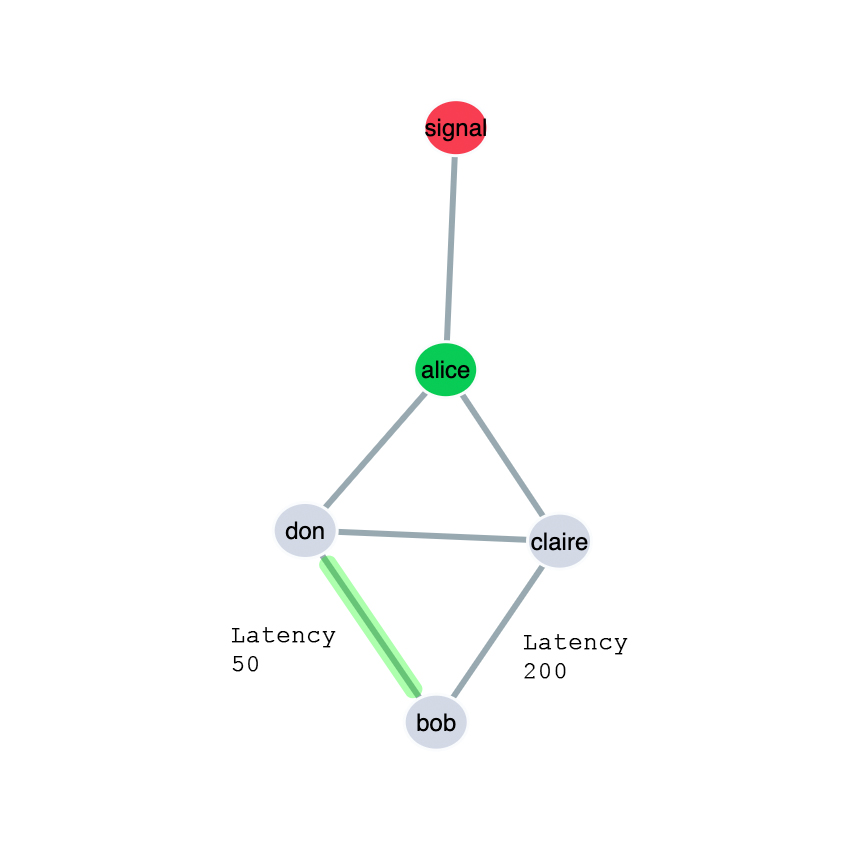
\includegraphics[width=0.25\textwidth]{graphics/analysis/mini-scenarios/send-message/2.jpg} \label{fig:filmstrips-send-message-b}}
	\subfloat[]{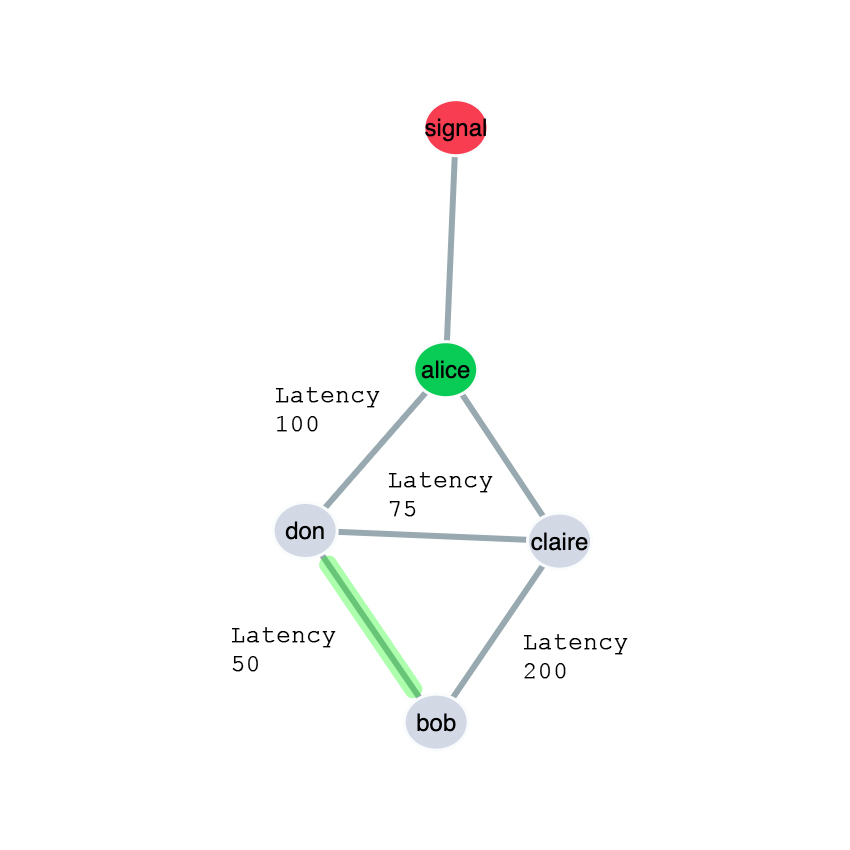
\includegraphics[width=0.25\textwidth]{graphics/analysis/mini-scenarios/send-message/3.jpg} \label{fig:filmstrips-send-message-c}}
	\subfloat[]{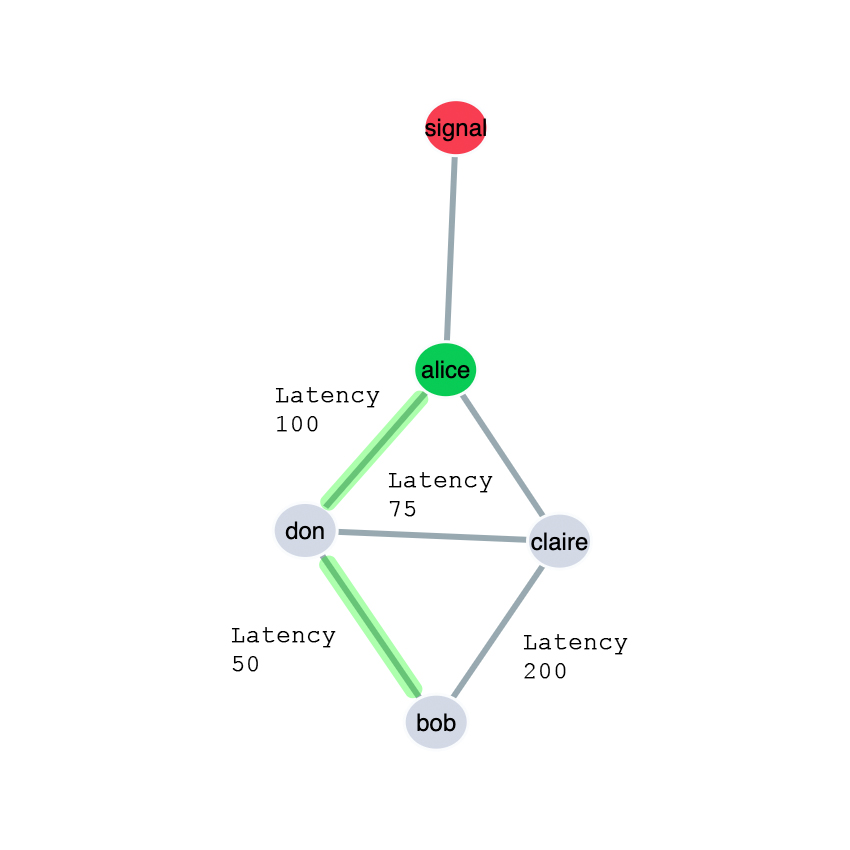
\includegraphics[width=0.25\textwidth]{graphics/analysis/mini-scenarios/send-message/4.jpg} \label{fig:filmstrips-send-message-d}}
	\caption{Path of a message}
\label{fig:filmstrips-send-message}
\end{figure}

Sending a message to another peer often means that multiple paths can be taken but only one of the paths is the best. \vref{fig:filmstrips-send-message-a} shows a scenario where \bob can choose between \don and \claire to send a message to \alice. \don has a millisecond latency of $l=50$ and \claire a latency of $l=200$, which \bob has measured by sending continuous ping messages and measuring the time until the pong message has been received.

Thus \bob is selecting \don to deliver the message (\vref{fig:filmstrips-send-message-b} to \alice as he has the best latency. 
\don is receiving the message. As the specified receiver address of the message is not his own address, he has to forward the message.

To forward the message he has two options: \claire with a measured latency of $l=75$ and \alice with a measured latency of $l=100$. He is selecting \alice as she is the designated receiver of the message even though the latency is worse (\vref{fig:filmstrips-send-message-c}).

\alice is receiving the message (\vref{fig:filmstrips-send-message-d}) and as her address matches the message receiver address, she is further processing the message.